\documentclass{beamer}
\usetheme{Madrid}
\usepackage[utf8]{inputenc}
\usepackage[czech]{babel}
\usepackage{hyperref}
\hypersetup{
    colorlinks=true,
    linkcolor=blue,
    filecolor=magenta,      
    urlcolor=blue,
}
\setbeamertemplate{navigation symbols}{}%remove navigation symbols


%Information to be included in the title page:
\title[Rozpoznávání RZ]{Mobilní aplikace pro rozpoznávání registračních značek vozidel}
\author[Stanislav Král]{Stanislav Král\\Vedoucí práce: Ing. Kamil Ekštein, PhD.}
\institute{Západočeská univerzita v Plzni\\Fakulta aplikovaných věd\\Katedra informatiky a výpočetní techniky}
\institute[FAV ZČU] % (optional)
{
Západočeská univerzita v Plzni\\
Fakulta aplikovaných věd\\
Katedra informatiky a výpočetní techniky
}
\date{2020}

\begin{document}

\frame{\titlepage}

\begin{frame}
\frametitle{Obsah prezentace}
\tableofcontents
\end{frame}


\section{Úvod}
\begin{frame}
\frametitle{Úvod}
\begin{itemize}
    \item nedostatek volně dostupného SW pro rozpoznávání registračních značek vozidel \textbf{mobilními telefony}
    \item nabídnout veřejnosti možnost postavit SW stavějící na této funkcionalitě
    \begin{itemize}
        \item evidence vozidel v autoservisech, placených parkovištích,...
        \item monitorování pohybu vozidel v dočasně zřízených kontrolních stanovištích
        \item pořizování důkazního materiálu při pojistných událostech
    \end{itemize}
\end{itemize}
\end{frame}

\section{Implementace}
\begin{frame}
    \frametitle{Implementace}
    \begin{columns}
    \column{0.7\textwidth}
    \begin{itemize}

        \item mobilní aplikace pro platformy Android a iOS vytvořená s využitím frameworku Flutter
        \item snímání scény fotoaparátem
        \item rozpoznávání RZ ve scéně realizováno pomocí OCR s kontrolou formátu identifikátoru
        \item naskenované RZ a dodatečné informace ukládané do lokální SQLite databáze
        \begin{itemize}
            \item adresa místa pořízení (buď ručně zadaná nebo automaticky dohledaná dle GPS souřadnic)    
            \item vlastní textová nebo hlasová poznámka
        \end{itemize}
    \end{itemize}
    \column{0.3\textwidth}
    {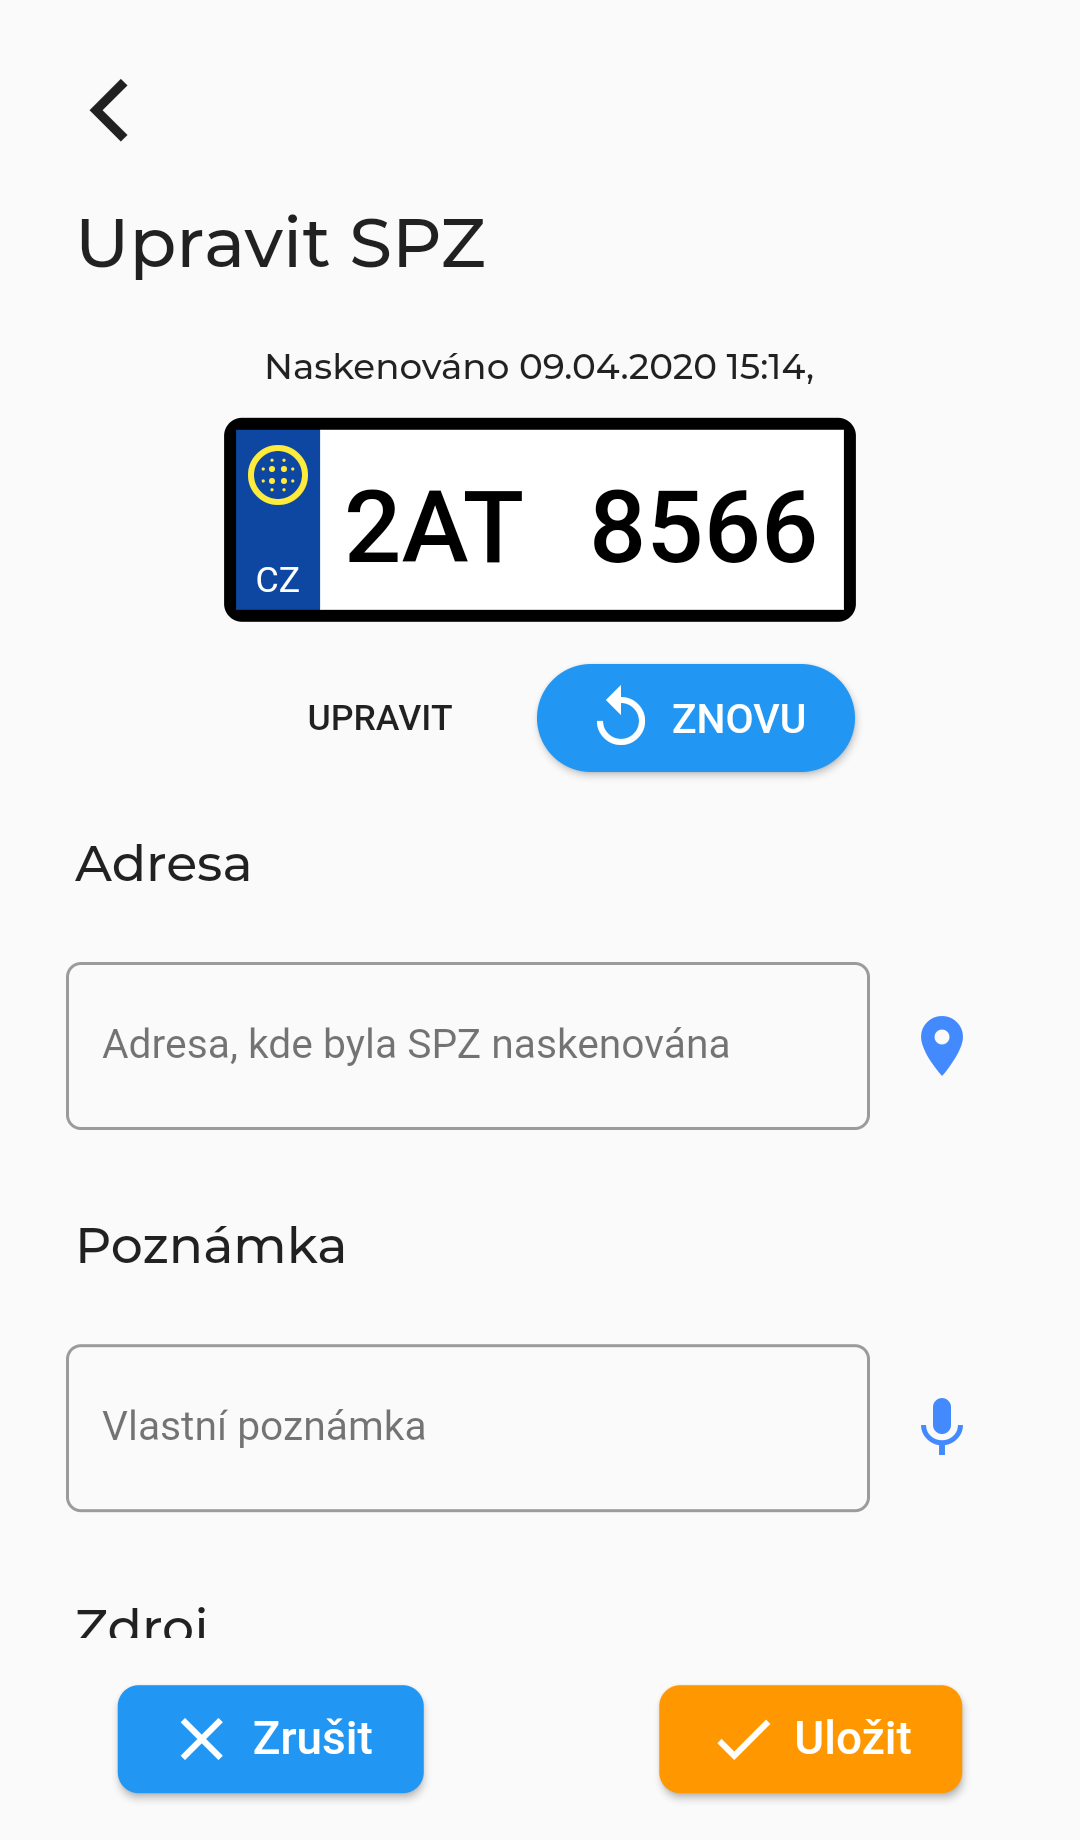
\includegraphics[width=2.8cm]{img/screen-preview.png}}

    \end{columns} 
\end{frame}

\begin{frame}
    \frametitle{Rozpoznávané RZ}
    \begin{columns}
    \column{0.7\textwidth}
    \begin{center}
    {
\includegraphics[width=6.8cm]{img/simple-vrp-czech.png}}
    \end{center}
    \begin{itemize}
        \item jednořádkové RZ
        \begin{itemize}
            \item klasické
            \item historické
            \item VIP
        \end{itemize}
        \item dvouřádkové RZ
        \begin{itemize}
            \item o rozměrech 340 $\times$ 200 mm
            \item RZ motocyklů
        \end{itemize}
    \end{itemize}
    \column{0.3\textwidth}
{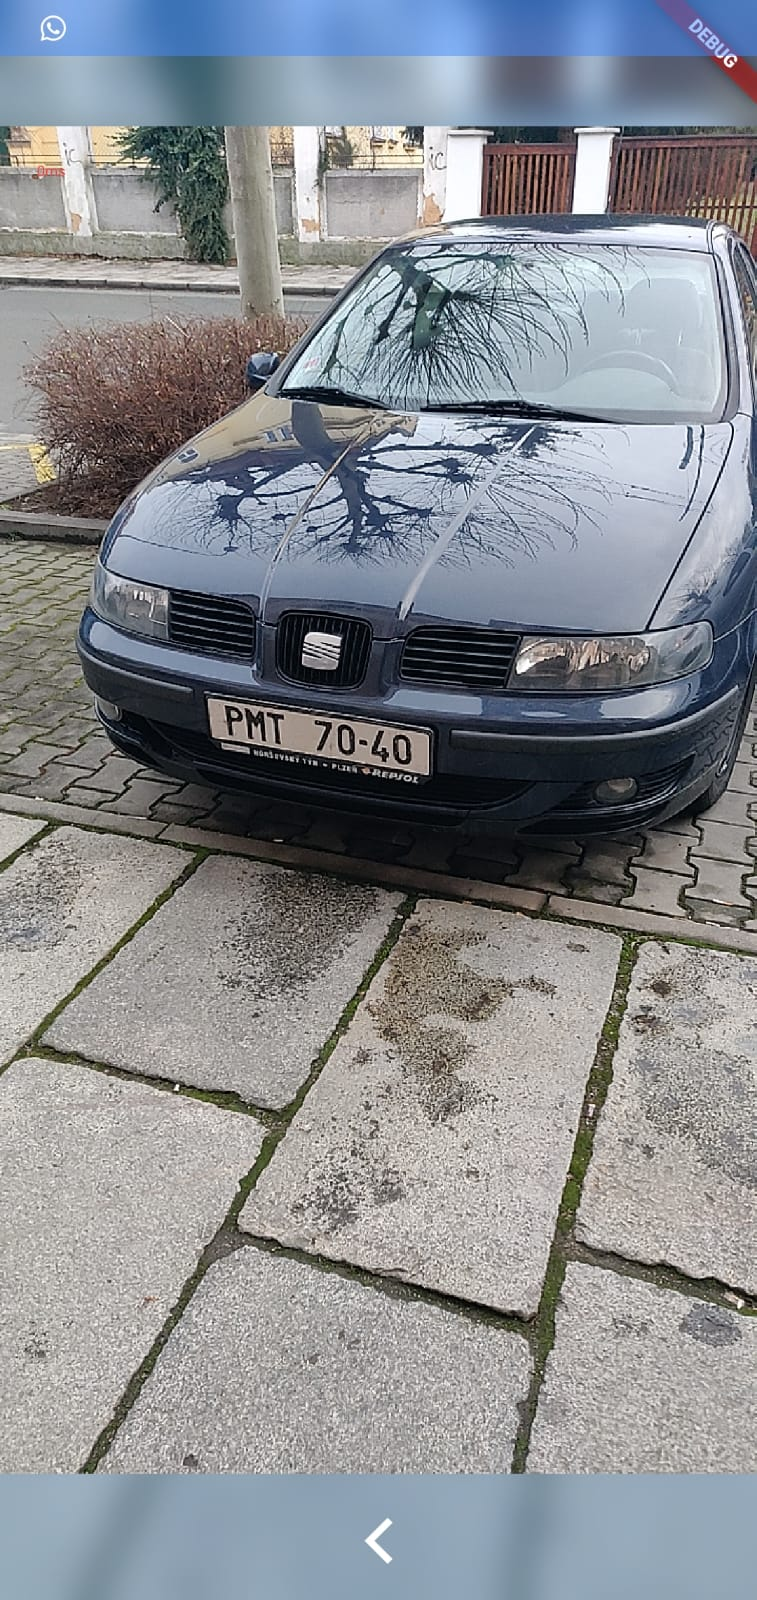
\includegraphics[width=2.8cm]{img/screen_2.jpeg}}

    \end{columns} 
\end{frame}

\begin{frame}
\frametitle{Diagram rozpoznávání RZ}
\begin{figure}[!ht]
\centering
{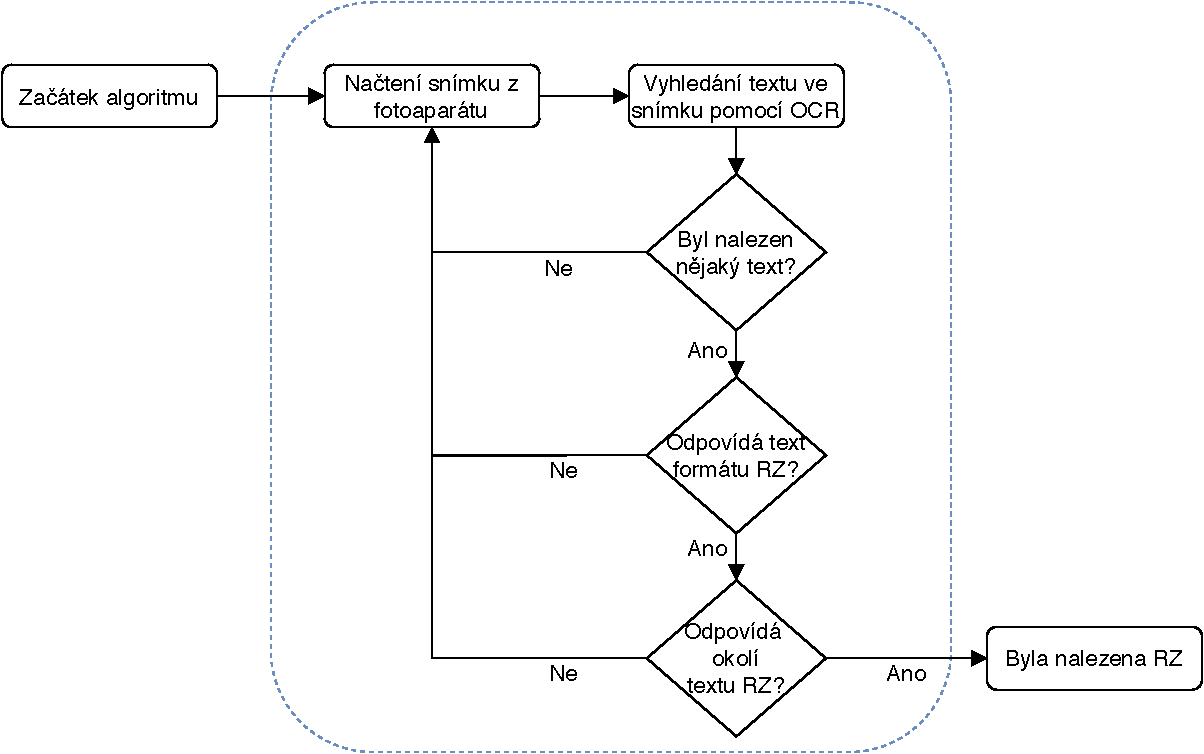
\includegraphics[width=11.5cm]{pdf/vrp_recognition.pdf}}
\end{figure}

\end{frame}

\section{Oprava chyby ve frameworku Flutter}
\begin{frame}
\frametitle{Oprava chyby ve frameworku Flutter}
\begin{itemize}
    \item během vývoje objevena chyba v balíčku \texttt{camera}
    \begin{itemize}
        \item snímání scény pomocí fotoaparátu se ne vždy chovalo korektně
        \item tato chyba se projevovala zřídka, čímž bylo její hledání ztížené
        \item někdy zapříčinila, že při skenování dvou různých aut byla v obou případech rozpoznána RZ prvního auta
    \end{itemize}
    \item bylo třeba analyzovat balíček \texttt{camera} z frameworku Flutter a chybu odhalit
    \item následně provést její opravu a vše řádně zdokumentovat
    \item vše nakonec předáno vývojářům tohoto frameworku pomocí služby \textbf{GitHub}\footnote{GitHub pull request - \url{https://github.com/flutter/plugins/pull/2655}}
\end{itemize}
\end{frame}

\section{Výsledky}
\begin{frame}
\frametitle{Výsledky práce}
\begin{itemize}
    \item rozšiřitelná \textbf{multiplatformní} mobilní aplikace rozpoznávající SPZ
    \item implementovaná metoda rozpoznávání je rychlá a přesná
    \item poradí si i se \textbf{zhoršenými světelnými podmínkami}
\end{itemize}

\pause

\begin{table}[!ht]
    \centering
        \begin{tabular}{| l | l | l | l | l | l | l | l | l |}
            \hline
            Galerie & P & FN & FP & $a$ & $\overline{a}$ & $t$ [ms] & $\overline{t}$ [ms] & Přesnost [\%]  \\ \hline \hline
            Slunečno & 21 & 0 & 0 & 33 & 1,57 & 6769 & 322  & 100 \\ \hline
            Zataženo & 5 & 0 & 0 & 7 & 1,40 & 1288 & 258  & 100 \\ \hline
            Podvečer & 17 & 1 & 0 & 30 & 1,67 & 6184 & 344  & 94,45 \\ \hline
            Večer & 19 & 3 & 1 & 52 & 2,26 & 10093 & 439  & 82,60 \\ \hline
        \end{tabular}
        \caption{\label{tab:table-name}Výsledky testování provedené na zařízení Oneplus 6.}
\end{table}

\pause

\begingroup
    \fontsize{8pt}{12pt}\selectfont
    \begin{itemize}
        \item \textbf{P} -- počet scénářů, ve kterých byla správně rozpoznána RZ
        \item \textbf{FN} -- počet scénářů, ve kterých nebyla rozpoznána žádná RZ
        \item \textbf{FP} -- počet scénářů, ve kterých byla nalezena nesprávná RZ
        \item \textbf{$a$} -- počet pokusů, které byly provedeny napříč scénáři
        \item \textbf{$t$} -- celkový čas rozpoznávání během celého testu
    \end{itemize}
\endgroup

\end{frame}

\begin{frame}
\frametitle{Závěr}
    \fontsize{14pt}{12pt}\selectfont
    \centering
    Děkuji vám za pozornost
\end{frame}


\begin{frame}
\frametitle{1. otázka z posudku oponenta}
    \begingroup
    \fontsize{11pt}{12pt}\selectfont
    \textit{Jak složité by bylo rozpoznávat více značek v jednom obrázku (např. při fotografii z parkoviště by bylo
vhodné rozpoznat i přehledovou fotografii)?}
    \endgroup
    \bigskip
    \begin{itemize}
        \item rozpoznávání nyní vybere RZ, která je nejblíže středu obrázku
            \begin{itemize}
                \item ostatní RZ zahodí
            \end{itemize}
        \item bylo by třeba:
        \begin{itemize}
            \item upravit rozhraní \texttt{VrpFinder} a jeho implementaci \texttt{VrpFinderImpl} tak, aby metoda \texttt{findVrpInImage()} vracela kolekci rozpoznaných RZ
            
            \item náležitě upravit UI aplikace

            \item dle další specifikace této funkcionality upravit databázi
        \end{itemize}
    \end{itemize}
\end{frame}

\begin{frame}

\frametitle{2. otázka z posudku oponenta}
    \begingroup
    \fontsize{11pt}{12pt}\selectfont
    \textit{Jaké úpravy by bylo potřeba učinit, aby aplikace rozpoznávala zahraniční registrační značky?}
    \endgroup
    \bigskip
    \begin{itemize}
        \item rozpoznávání RZ je závislé na kontrole formátu identifikátoru RZ 
        \item bylo by třeba:
        \begin{itemize}
            \item implementovat rozhraní \texttt{VrpValidator}, které validuje rozpoznané textové bloky ve snímku  
            \item po implementaci tohoto rozhraní přidat jeho instanci do kolekce používaných validátorů ve třídě \texttt{VrpFinderImpl}

            \item dle další specifikace této funkcionality upravit UI
        \end{itemize}
    \end{itemize}
\end{frame}

\begin{frame}
\frametitle{3. otázka z posudku oponenta}
    \begingroup
    \fontsize{11pt}{12pt}\selectfont
    \textit{V textu práce je zmiňována multiplatformnost řešení. Jaké další kroky by bylo potřeba podniknout?}
    \endgroup
    \bigskip
    \begin{itemize}
        \item aplikace je připravená k sestavení na obě hlavní mobilní platformy \textbf{Android} a \textbf{iOS}
        \item aplikace byla důkladně otestována na široké škále zařízení s Android OS
        \item kvůli koronavirové situaci nebylo možné použít ve školní laboratoři zařízení s \textbf{macOS}, provést sestavení pro iOS a následně zde aplikaci otestovat 
        \begin{itemize}
            \item aplikace by však v aktuálním stavu měla být zcela funkční i na platformě iOS
            \item bylo by třeba otestovat, zdali korektně funguje zpracování snímků ve formátu používaným na platormě iOS 
            \item ostatní funkční kód je identický pro obě platformy, a tudíž by nebylo třeba provádět další úpravy 
        \end{itemize}
    \end{itemize}
\end{frame}

\begin{frame}
\frametitle{4. otázka z posudku oponenta}
    \begingroup
    \fontsize{11pt}{12pt}\selectfont
    \textit{Provedl jste průzkum trhu, zda neexistují nějaké podobné aplikace pro Android?}
    \endgroup
    \bigskip
    \begin{itemize}
        \item ve službě \textbf{Google Play} mnoho aplikací určených k rozpoznávání RZ není
            \begin{itemize}
                \item aplikace \textbf{Mobile LPR}, podporující RZ spoustu zemí včetně ČR
                \item aplikace \textbf{Automatic License Plate Recognition Feature} podporující některé státy USA a Evropy (\textbf{ČR nepodporována})
                \item většina aplikací vyhledává informace o vozidle dle \textbf{ručně zadané} RZ
            \end{itemize}
        \item komerční placená aplikace \textbf{Licence Plate Reader} od firmy \textbf{Z&G}

        \item další mobilní aplikace pro tuto platformu se mi nepodařilo najít
    \end{itemize}
\end{frame}


\end{document}
